\documentclass{astroedu-lab}

\begin{document}

\pagestyle{plain}

\begin{problem}{\huge Лабораторная работа 1.4.5\\\\Изучение колебаний струны\\\\Выполнил Жданов Елисей Б01-205}

\section{Цель работы:}

1) Изучить поперечные стоячие волн на тонкой натянутой струне

2) Измерить собственные частоты колебаний струны и проверить условие образования стоячих волн

3) измерить скорость распространения поперечных волн на струне и исследовать её зависимость от натяжения струны

\section{Оборудование:}

1) Закрепленная на станине стальная струна

2) Набор грузов

3) Электромагнитные датчики

4) Звуковой генератор 

5) Двухканальный осциллограф

6) Частотомер

\section{Теория колебаний струны:}

Рассмотрим гибкую однородную струну, в которой создано натяжение T, и получим дифференциальное уравнение, описывающее её малые поперечные свободные колебания. Отметим, что, если струна расположена горизонтально в поле тяжести, величина T должна быть достаточна для того, чтобы в состоянии равновесия струна не провисала, т.е. сила натяжения должна существенно превышать вес струны.

\newpage

Направим ось $x$ вдоль струны в положении равновесия. Форму струны
будем описывать функцией $y$($x$, $t$), определяющей её вертикальное смещение в точке $x$ в момент времени $t$ (см. рис. 1). Угол наклона касательной к струне в точке $x$ относительно горизонтального направления обозначим как $\alpha$. В любой момент этот угол совпадает с углом наклона касательной к графику функции $y(x)$, то есть $\tan{\alpha} = \frac{\delta y}{\delta x}$.
\begin{center}
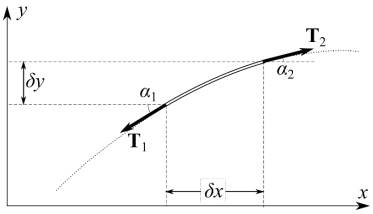
\includegraphics[width=0.6\textwidth]{theory_1.png}
\label{ris:image}
\end{center}

Рассмотрим элементарный участок струны, находящийся в точке $x$ ,
имеющий длину $\delta x$ и массу $\delta m = \rho_l \delta x$, где $\rho_l$ [кг/м] — погонная плотность струны (масса на единицу длины). При отклонении от равновесия на выделенный элемент действуют силы натяжения T1 и T2, направленные по касательной к струне. Их вертикальная составляющая будет стремиться вернуть рассматриваемый участок струны к положению равновесия, придавая элементу некоторое вертикальное ускорение$\frac{\delta^2 y}{\delta t^2}$. Заметим, что угол $\alpha$ зависит от координаты $x$ вдоль струны и различен в точках приложения сил T1 и T2. Таким образом, второй закон Ньютона для вертикального движения элемента струны запишется в следующем виде

\begin{equation}
	\delta m \frac{\delta^2 y}{\delta t^2} = -T_1 \sin{\alpha_1} + T_2 \sin{\alpha_2}
\end{equation}

Основываясь на предположении, что отклонения струны от положения
равновесия малы, можем сделать ряд упрощений


1) Длина участка струны в смещенном состоянии практически равна
длине участка в положении равновесия, поэтому добавочным
напряжением вследствие удлинения струны при деформации можно пренебречь.  Следовательно, силы T1 и T2 по модулю равны силе
натяжения струны: $T_1 \approx T_2 \approx T$

2) Углы наклона $\alpha$ малы, поэтому $\tan{\alpha} \approx \sin{\alpha} \approx \alpha$, и, следовательно, можно положить $\alpha \approx \frac{\delta^2 y}{\delta t^2}$.

Разделим обе части уравнения движения на $\delta x$ и устремим размер элемента к нулю, $\delta x \rightarrow 0$. Тогда правая часть (1) примет вид

\begin{equation}
	\rho_l \frac{\delta^2 y}{\delta t^2} = \frac{T_2 \sin{\alpha} - T_1 \sin{\alpha}}{\delta x} \approx T \frac{\alpha_2 - \alpha_1}{\delta x} \rightarrow T \frac{\delta \alpha}{\delta x}
\end{equation}

Наконец, подставляя $\alpha = \frac{\delta y}{\delta x}$ и вводя величину с размерностью скорости

\begin{equation}
	\boxed{u = \sqrt{\frac{T}{\rho_l}}}
\end{equation}

находим окончательно уравнение свободных малых поперечных колебаний
струны

\begin{equation}
	\frac{\delta^2 y}{\delta t^2} = u^2 \frac{\delta^2 y}{\delta x^2}
\end{equation}

Это уравнение называют волновым уравнением.

Найдем вид свободных колебаний струны с закрепленными концами.
Пусть струна закреплена в точках $x = 0$ и $x = L$. Концы струны не колеблются, поэтому $y(0, t) = 0$ и $y(L, t) = 0$ для любых t.

Из формулы

\begin{equation}
	y(0, t) = a \cos{\omega t} + b \cos{\omega t} = 0
\end{equation}

следует, что $a = -b$. Тогда после тригонометрических преобразований выражение примет вид

\begin{equation}
	y(x, t) = 2 a \sin{k x} \cdot \sin{\omega t}
\end{equation}

Колебания струны, описываемые функцией, называются стоячими волнами. Видно, что стоячая волна может быть получена как суперпозиция двух гармонических бегущих навстречу друг другу волн с равными амплитудами.

Как видно из формулы, точки струны, в которых $\sin{k x} = 0$, в любой момент времени неподвижны. Такие точки называются узлами стоячей волны. Остальные участки струны совершают в вертикальной плоскости гармонические колебания с частотой $\nu = \frac{\omega}{2 \pi} = \frac{u}{\lambda}$. Амплитуда колебаний распределена вдоль струны по гармоническому закону: $y_0(x) = 2 a \sin{k x}$. В точках,
где $\sin{k x}$, амплитуда колебаний максимальна, такие точки называются пучностями. Между двумя соседними узлами все участки струны колеблются в фазе (их скорости имеют одинаковое направление), а при переходе через узел фаза колебаний меняется на $\pi$ вследствие изменения знака $\sin{k x}$.

Используя второе граничное условие $y(L, t) = 0$ (точки крепления струны должны быть узлами стоячей волны), найдём условие образования стоячих волн на струне $y(x, t) = 2 a \sin{k L} \sin{\omega t} = 0$, откуда

\begin{equation}
	\sin{k L} = 0 \rightarrow k L = n \frac{\pi}{2}
\end{equation}

Причем n натуральное. Таким образом, стоячие волны на струне с закреплёнными концами образуются, только если на длине струны укладывается целое число полуволн

\begin{equation}
	\boxed{\lambda_n = \frac{2 L}{n}}
\end{equation}

На рисунке показана картина стоячих волн для n = 1, 2, 3. Заметим, что число n определяет число пучностей (но не узлов!) колеблющейся струны. Поскольку длина волны однозначно связана с её частотой, струна может колебаться только с определёнными частотами

\begin{equation}
	\nu_n = \frac{u}{\lambda_n} = \frac{n}{2 L} \sqrt{\frac{T}{\rho}}
\end{equation}

Набор (спектр) разрешённых частот $\nu_n$ называют собственными частотами колебаний струны. Режим колебаний, соответствующий каждой из частот $\nu_n$, называется собственной (или нормальной) модой колебаний (от англ. mode — режим). Произвольное колебание струны может быть представлено в виде суперпозиции её собственных колебаний. Наименьшая частота $\nu_1$ называется также основным тоном (или первой гармоникой), а остальные ($\nu_2$ = 2 $\nu_1$, $\nu_3$ = 3 $\nu_1$) — обертонами (высшими гармониками). Здесь термин гармоника мы употребляем в обобщенном смысле - как элементарную гармоническую составляющую сложного колебательного процесса.

\begin{center}
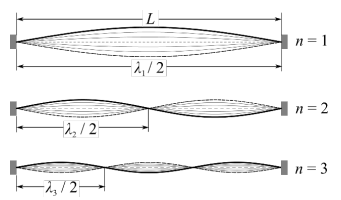
\includegraphics[width=0.6\textwidth]{theory_2.png}
\label{ris:image}
\end{center}

Таким образом, спектр собственных частот тонкой струны определён её погонной плотностью $\rho_l$ , внешней силой натяжения T и длиной
струны L и не зависит от модуля Юнга материала струны.

При колебаниях реальной струны всегда имеет место потеря энергии
(часть теряется вследствие трения о воздух; другая часть уходит через неидеально закрепленные концы струны и т.д.). Поддержание незатухающих колебаний в струне может осуществляться точечным источником, в качестве которого в данной работе используется электромагнитный вибратор.

Для эффективной раскачки колебаний используется явление резонанса - вынуждающая частота $\nu$ должна совпадать с одной из собственных частот струны $\nu_n$ (в этом смысле струна аналогична обычной колебательной системе, например маятнику или грузу на пружине, только вместо единственной собственной резонансной частоты струна обладает бесконечным спектром резонансных частот $\nu_n$). Когда потери энергии в точности компенсируются энергией, поступающей от вибратора, колебания струны становятся стационарными и на ней можно наблюдать стоячие волны.

Замечу, что для достижения максимального эффекта возбуждающий датчик следует располагать вблизи узловой точки. 

\section{Описание установки:}

Стальная гитарная струна 1 закрепляется в горизонтальном положении между двумя стойками с зажимами 2 и 3, расположенными на массивной станине 4. Один конец струны закреплен в зажиме 2 неподвижно. К противоположному концу струны, перекинутому через блок, прикреплена платформа с грузами 5, создающими натяжение струны. Зажим 3 можно передвигать по станине, устанавливая требуемую длину струны. Возбуждение и регистрация колебаний струны осуществляются с помощью электромагнитных датчиков (вибраторов), расположенных на станине под струной. Электромагнитный датчик 6 подключен к звуковому генератору 7 и служит для возбуждения колебаний струны, частота которых измеряется с помощью частотомера 10 (в некоторых установках частотомер встроен в генератор). Колебания струны регистрируются с помощью электромагнитного датчика 8, сигнал с которого
передается на вход осциллографа 9. Разъёмы, через которые датчики с помощью кабелей соединяются с генератором и осциллографом, расположены на корпусе станины. 

\begin{center}
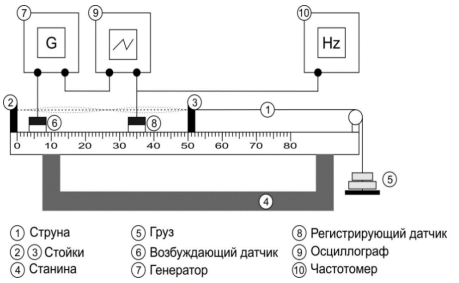
\includegraphics[width=0.6\textwidth]{state.png}
\label{ris:image}
\end{center}


\section{Измерения:}

1) Убедимся, что установка заранее отлично откалибрована. Это впоследствии можно будет заметить по добротности колебаний.

2) Начну измерения с 2 грузов

\begin{equation}
	u = \sqrt{\frac{T}{\rho}} = \sqrt{\frac{1.102 \cdot 9.81}{568.4 \cdot 10^{-6}}} \approx 138 \text{ Гц}
\end{equation}

Зафиксировав длину активой части проволки $L = 50$ см, буду использовать её в расчетах на протяжении всего эксперимента.

Частота, соответствующая такой скорости распространения

\begin{equation}
	\nu = \frac{u}{\lambda} = 138 \text{ Гц}
\end{equation}

3) Включим все требуемое оборудование

4) Добьемся высоких резонансных амплитуд при первом запуске

Частота составляет 137.9 см, что считаю замечательным результатом.

5) Убежусь в визуальной наблюдаемости резонанса, подкрепляя замеры с помощью осциллографа. Также замечу, что на больших гармониках слышен звук от колебаний струны.

6 - 7) Включу осциллограф и проверю его требуемую функциональность.

8 - 10) Занесу все данные в таблицу(стартовая масса: $m_0 = 1102.2$ г)

\begin{center}
\begin{tabular}{|c|c|c|c|c|c|c|}
\hline n & \multicolumn{6}{|c|}{$\nu$, Гц} \\ \hline
$m_i+$г & 000.0 & 450.9 & 450.2 & 461.7 & 493.0 & 338.0	\\ \hline
1 & 137.9 & 163.5 	 & 185.3 & 201.8 & 221.3 & 233.4   	\\
2 & 278   & 327		 & 372   & 405   & 443   & 468  	\\
3 & 415   & 492 	 & 557   & 606   & 664   & 701  	\\
4 & 553   & 658		 & 742	 & 810	 & 888	 & 935		\\
5 & 694	  & 821   	 & 930   & 1013  & 1109  & 1169 	\\
6 & 831	  & 983	 	 & 1116	 & 1218	 & 1334	 & 1407		\\
7 & 975   & 1153	 & 1304	 & 1419	 & 1554	 & 1639		\\
8 & 1124  & 1315	 & 1491	 & 1628  & 1781	 & 1880		\\
9 & 1261  & 1489	 & 1682	 & 1828	 & 2002  & 2111		\\
\hline
\end{tabular}
\end{center}

Для четных гармоник необходимо передвигать датчик, благо, это довольно просто рассчитать.

11) Выставлю частоту, половину от 137.9. Добившись резонанса, наблюдаю следующую картину

\begin{center}
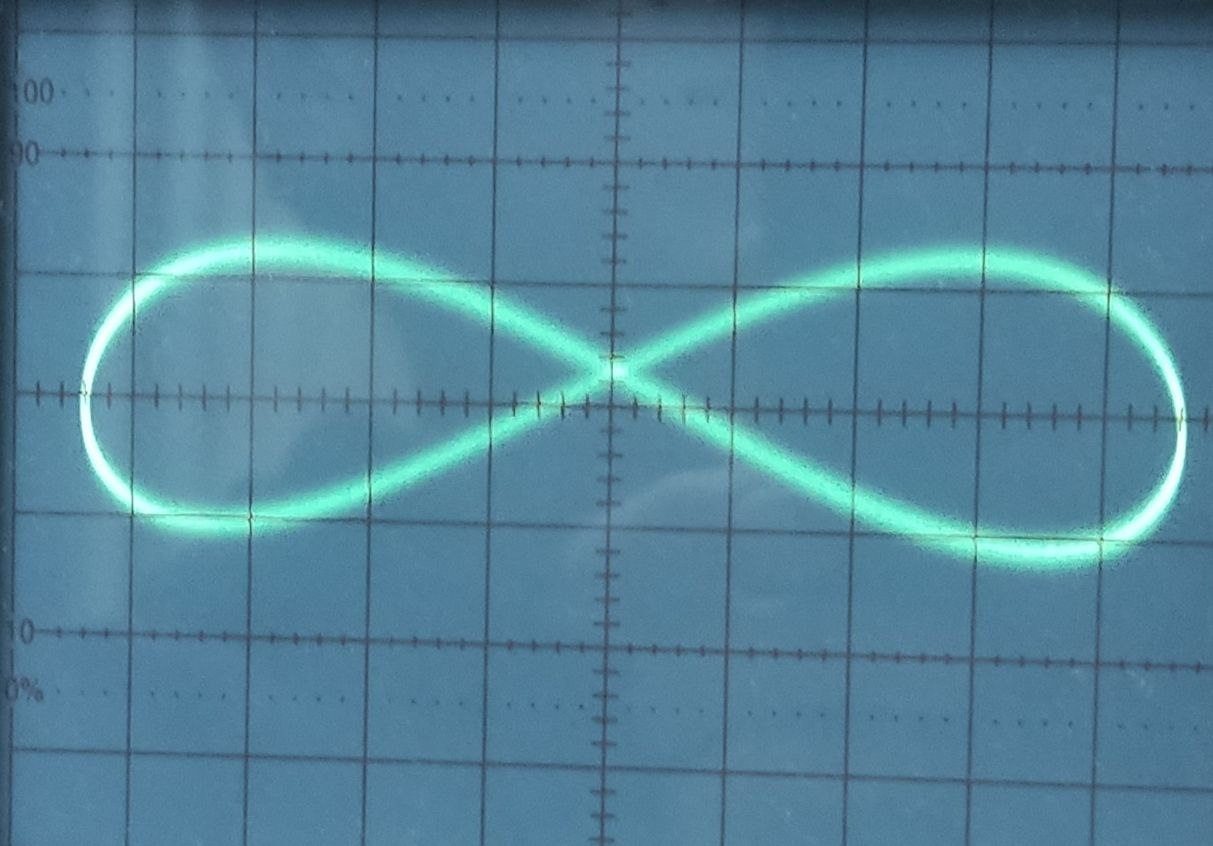
\includegraphics[width=0.6\textwidth]{res.jpg}
\label{ris:image}
\end{center}

Очень четкая фигура Лиссажу. Проведу замеры для других кратных частот(увы, резонанс хорошо ловится только на паре следующих, недостаточная добротность при десятках герц дает о себе знать), для них фигуры лиссажу будут выглядить подобным образом, только самопересечений будет соотвествующее число.

12) Увы, данные о добротности весьма обрывочные и оценочные, но постараюсь достоино их обработать.

\begin{center}
\begin{tikzpicture}
\begin{axis}[
	width=300,
	ymin = 0,
	ylabel     = \text{$A$},
    xlabel     = \text{$\nu$ [Гц]},
	]
\addplot[mark = *] table {
	x     y
216.8 3
216.7 2
216.6 1.5
216.5 1
};

\end{axis}
\end{tikzpicture}
\end{center}

Собственно, полуширине соответствует приблизительно значение 0.1 Гц, если считать, что 3 соотвествует маскимальная амплитуда. Тогда добротность составляет

\begin{equation}
	Q = \frac{\nu_res}{\Delta \nu} = \frac{216.8}{0.2} = 1000
\end{equation}

Чтож, сделаю вывод о добротности в соответствующей графе.

\section{Обработка:}


13) Визуально(а точнее акустически) просто определять резонансную частоту. Поэтому неудивительно, что замеры обоими способами дают одинаковые результаты. Это говорит о замечательной точности подобной методики и немного о точности приборов и экспериментатора.

14) Буду считать исходную массу $m_0 = 1102.2$ г. Нанесу все прямые на один график.

\begin{center}
\begin{tikzpicture}
\begin{axis}[
	width=500,
	xmin = 0, ymin = 0,
	ylabel     = \text{$\nu$ [Гц]}, % label x axis
    xlabel     = \text{$n$}, % label y axis
	]
\addplot[mark = *] table {
	x     y
1 137.9
2 278  
3 415  
4 553  
5 694	 
6 831	 
7 975  
8 1124 
9 1261 
0 0
};
\addplot[mark = *] table {
	x     y
1 163.5 	
2 327		
3 492 	
4 658		
5 821   	
6 983	 	
7 1153	
8 1315	
9 1489	
0 0
};
\addplot[mark = *] table {
	x     y
1 185.3
2 372  
3 557  
4 742	
5 930  
6 1116	
7 1304	
8 1491	
9 1682
0 0
};	
\addplot[mark = *] table {
	x     y
1 201.8
2 405  
3 606  
4 810	
5 1013 
6 1218	
7 1419	
8 1628 
9 1828	
0 0
};
\addplot[mark = *] table {
	x     y
1 221.3
2 443  
3 664  
4 888	
5 1109 
6 1334	
7 1554	
8 1781	
9 2002 
0 0
};
\addplot[mark = *] table {
	x     y
1 233.4   
2 468  
3 701  
4 935	
5 1169 
6 1407	
7 1639	
8 1880	
9 2111
0 0
};
\end{axis}
\end{tikzpicture}
\end{center}

Кресты погрешностей не нанесены, поскольку ей можно пренебречь в рамках масшаба графика.

Как видно, все прямые хорошие)

Рассчитаю коэффициенты наклона имеющихся прямых, и посколько они численно равны скорости распространения волны($2 L = 1.000 \pm 0.001$ м), сделаю итоговую таблицу

\begin{center}
\begin{tabular}{|c|c|c|}
\hline u, м/c & $m_i$, г & T, Н \\ \hline
$(139.0 \pm 0.3)$ & 1102.2 & 10.81 \\
$(164.2 \pm 0.2)$ & 1553.1 & 15.24 \\
$(186.0 \pm 0.2)$ & 2003.3 & 19.66 \\
$(202.6 \pm 0.2)$ & 2465.0 & 24.19 \\
$(221.9 \pm 0.2)$ & 2958.0 & 29.03 \\
$(234.1 \pm 0.2)$ & 3296.0 & 32.35 \\
\hline
\end{tabular}
\end{center}

Погрешность состоит из случайной погрешности измерения частот и погрешности L.

16) Здесь лучше построю график на основе вычисленных значений u

\begin{center}
\begin{tikzpicture}
\begin{axis}[
	width=500,
	xmin = 0, ymin = 0,
	ylabel     = \text{$u^2$ [м$^2$/c$^2$]}, % label x axis
    xlabel     = \text{$T$ [Н]}, % label y axis
	]
\addplot[mark = *, only marks] table {
	x     y
10.81 19321
15.24 26961
19.66 34596
24.19 41047
29.03 49240
32.35 54803
};
\addplot[mark = ] table {
	x     y
0 1958
32 54175
};
\end{axis}
\end{tikzpicture}
\end{center}

Итоговое значение погонной плотности

\begin{equation}
	\rho = (613 \pm 6) \text{ мг / м}
\end{equation}

Вывод о различие ниже.

\section{Время делать выводы:}

По прошествии работы могу утверждать, что было проведено полное исследование колебаний струны.

Добротность струны оказалась довольно высокой, для подобной системы измеряемые частоты не должны быть много больше добротности. Это правда, максимальная частота в 2 раза превосходит значение Q, поэтому порядка долей секунды струна продолжит совершать колебания после отключения питания, что весьма хорошо.

Также были исследованы фигуры Лиссажу для кратных частот; могу заметить, что при маленькой частоте премя затухания становится сравнимо с частотой, поэтому резонанс трудно поймать. Тем не менее, наблюдение 2 фигур Лиссажу считаю достаточным для подтверждения теоретической модели явления.

Итоговое значение погонной плотности не критично, но заметно отличается от нормировочного($613 = 568 \pm 8\%$). Это можно объяснить тем, что замер с помощью весов обладает своими систематическими издержками и вообщем-то меряет не то, что нужно. Акустическая погонная плотность включает в себя специфику формы, профиля и точности проволки. Погонная плотность же усредняет это. Отличие в 8 процентов приемлемое для 2-х таких замеров.

Приблизим работу выполненной.


\end{problem}
\end{document}
